\section{Internet Telephony}
\label{sec:measurement:voip}

We have seen in 
Section~\ref{subsec:related:voip-qoe} that user 
experience is sensitive to poor network performance 
and that a significant fraction of calls suffer from poor 
performance when using \direct routing. 

In this section, we use production data from a large VoIP service 
provide \skype (same dataset described in
 Section~\ref{subsec:related:voip-qoe}) 
to understand the QoE problems in Internet telephony
based on a similar spatial and temporal analysis used in the last section.
We begin by describing the dataset, QoE metrics, and the methodology
of analyzing spatial and temporal patterns
of VoIP QoE problems (Section~\ref{subsec:measurement:voip:method}),
and present our results in 
Section~\ref{subsec:measurement:voip:spatial}, 
~\ref{subsec:measurement:voip:temporal}, and
~\ref{subsec:measurement:voip:correlation}.
%and finally discuss the key takeaways in 
%Section~\ref{subsec:measurement:voip:discuss}
%quantify the impact of network metrics on 
%audio call quality, and patterns of poor network performance. 
%The observations motivate the need for and the design 
%requirements of \hybrid.


%{\em How well does PNR on average values compare to 
%using full packet traces?} 
%Analysis of a subset of ($70$K) calls with full packet traces 
%shows that $80\%$ of calls rated ``non-poor'' using the 
%thresholds on average metrics (``at least one poor metric'') 
%have a (packet-trace based) MOS score higher than 
%three-quarters ($75\%$) of calls rated ``poor'' using the 
%average metrics. We run a proprietary MOS calculator 
%on the packet traces that contain send/receive timestamps 
%for each packet and loss information. 
%This shows that defining the thresholds on average values 
%of the call is a reasonable approximation.

\subsection{Methodology}
\label{subsec:measurement:voip:method}

\mypara{Identifying bad QoE}
First, we define bad VoIP QoE by a similar threshold-based method
as we defined problem sessions in video.
We define the {\em poor network rate} (PNR) of a network 
metric for a set of calls as the fraction of calls whose performance 
on the metric is worse than the chosen thresholds: 
RTT $\geq 320$ms, loss rate $\geq 1.2\%$, jitter $\geq 12$ms. 
Recall from Figure~\ref{fig:perf-cdf} that these thresholds 
correspond to the user-specified poor call rate (PCR) of $0.3$.
These values are in line with literature from industry 
and standards bodies that recommend one-way end-to-end 
delay of no more than $150$ ms and a packet loss rate of 
no more than $1\%$ for good call quality~\cite{cisco-voip, itu}. 

\mypara{Clustering calls}
Similarly to video streaming, we would like to understand whether
the calls with bad network performance concentrate spatially 
(e.g., are they mostly International calls?) and persist
over time. To this end, we group calls in the dataset based on 
different spatial features (e.g., geo-locations and IP prefixes 
of the caller and callee) as well as time-stamp (the date in which
the call was made).


%Next, we analyze whether the calls with poor networks 
%share common patterns. This subsection focuses on 
%{\em spatial} patterns while
%Section~\ref{subsec:measurement:voip:temporal} 
%looks at {\em temporal} patterns.

\subsection{Spatial Patterns}
\label{subsec:measurement:voip:spatial}



% We define the {\em poor network rate} (PNR) for a given set of calls as the fraction of calls whose network performance is worse than the thresholds: RTT $\geq 320$ms, loss rate $\geq 1.2\%$, jitter $\geq 12$ms. PNR can be measured both on the individual metrics (how often were each of them poor?) as well as collectively (how often was {\em at least one} of the metrics poor?). Recall from Figure~\ref{fig:perf-cdf} that these thresholds correspond to the user-specified poor call rate (PCR) of $0.3$.
% to poor call performance with a probability of $0.5$. 

\begin{figure}[t!]
\centering
\subfloat[\small{International vs. domestic}]
{
        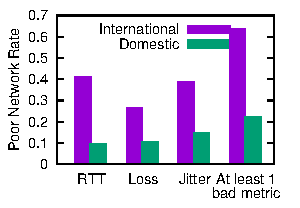
\includegraphics[width=0.45\textwidth]{figures/Via-Opportunity-International.pdf}
        \label{subfig:opportunity-international}
}
\subfloat[\small{Countries of one side of a call}]
{
        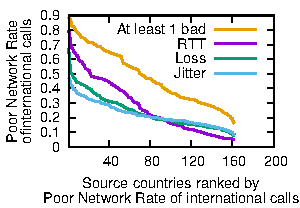
\includegraphics[width=0.45\textwidth]{figures/Via-Opportunity-International-ByCountry.pdf}
        \label{subfig:international-bycountry}
}
\caption{International vs. Domestic Calls.}
\label{fig:country}
\end{figure}

\mypara{International vs. domestic calls} 
On all three network metrics, we see that international 
calls (between users in different countries) have a
 higher PNR, i.e., they are more likely to suffer from 
 bad network performance than domestic calls. 
Figure~\ref{fig:country} shows a $2-3\times$ higher 
PNR on international calls than on domestic calls. 
The figures also show the fraction of calls with at least 
one metric being poor (the last pair of bars), where the 
gap between international and domestic calls is even 
larger. 
Though conclusively diagnosing the root cause of bad 
performance on international calls is hard and beyond 
the scope of this work, the higher PNR for international 
calls points to the WAN path as the culprit.\footnote{One 
aspect is that users tend to use VoIP 
regardless of its performance for international calls, 
unlike domestic calls.} %\cmrvnp{we speculate that it is because ISPs have less incentive to ensure good quality for international calls than domestic ones.}}

% \vnp{The "at least 1 bad metric" bars seem at least as tall as the other bars stacked up, which suggests that there is little overlap between the subsets for which each metric is poor.}

To understand this further, 
Figure~\ref{subfig:international-bycountry} zooms into 
the international calls and classifies them by the country 
of the callers (source). 
We see that there is a skewed distribution, with certain 
countries having a PNR as high as on the individual metrics. 
The PNR of international calls across the remaining 
countries drops gradually but half of them still see a 
non-negligible PNR of $25\%-50\%$. 
This suggests that poor network performance is 
quite widespread, highlighting the suitability of a 
{\em globally} deployed overlay network that provides 
high performance inter-connection between overlay nodes.
% and calling for a selective approach to routing via the managed network. 
% but the overall distribution is flat, indicating that most countries do not have particularly poor network performance. 

\begin{figure}[t!]
\centering
%\hspace{-0.5cm}
\subfloat[Inter-domain vs. intra-domain]
{
        \includegraphics[width=0.45\textwidth]{figures/Via-Opportunity-Interdomain.pdf}
        \label{subfig:opportunity-interdomain}
}%\hspace{-0.5cm}
\subfloat[Source AS]
{
        \includegraphics[width=0.45\textwidth]{figures/Via-Opportunity-Interdomain-ByAs.pdf}
        \label{subfig:interdomain-byas}
}%\hspace{-0.5cm}
\caption{Inter-domain vs. intra-domain calls.}
\label{fig:domain}
\end{figure}

\mypara{Inter-AS vs. intra-AS calls} % The above trends persist when we splice calls by the AS domains of the source and destinations. 
Similar to international calls, calls across ASes 
are $2-3\times$ more likely to experience poor 
network performance than those within the same 
AS domain. %Also, while calls originating from a small fraction of the ASes have a much higher PNR, the overall distribution is even. 
%This, again, points to the need for a selective approach to routing via the global managed overlay.
This, again, points to the need for enabling alternatives to default routing to improve WAN performance.
% a relay system that provides wide-area routing of better performance.

\begin{figure}[t!]
\centering
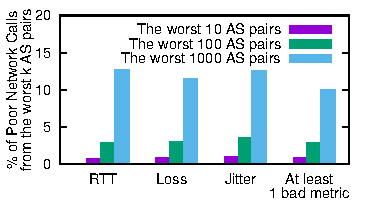
\includegraphics[width=0.6\textwidth]{figures/Via-BadContribution-Top-AsPair.pdf}
\caption{The percentage of calls over poor network 
conditions that come from the worst $n$ AS pairs; 
AS-pairs are ranked in descending order of their 
contribution to total amount of calls with poor performance.}
 %\ga{Change ``top'' to ``worst''.}
\label{fig:bad-contribution}
\end{figure}

\mypara{Not just a few problematic source-destination pairs}
Contrary to our expectation, a few source-destination pairs 
alone do {\em not} account for a big chunk of the PNR. % Our hypothesis was to observe the commonly occurring ``Pareto'' effect.
 Figure~\ref{fig:bad-contribution} shows the fraction of 
 calls that suffer from poor network performance from the 
 worst AS pairs, ranked in order of their contribution to the 
 overall PNR. %Across different metrics, we see that the calls with poor network metrics are not limited to a handful of AS pairs. 
Even the worst $1000$ AS pairs together only count for less 
than $15\%$ of the overall PNR. %\vnp{I'm unable to reconcile these numbers with the bars depicted in Fig 5.} 
This means that localized solutions that fix a few bad ASes 
or AS pairs, e.g., informing the AS administrators or the 
clients directly regarding their ISPs, are not sufficient. 
 
%\vnp{Absolute counts don't quite tell the full story. We should also report what fraction of all AS pairs seen is represented by k}
 
While the above analysis was at the granularity of ASes, 
we also tested at other, finer granularities (e.g., $/24$ and 
$/20$ prefixes of the caller and callee IP addresses) and 
found similar results (of not just a few culprits).
In fact, for the pairs with sufficient data density at the $/24$ 
granularity, we found that performance distributions of the 
network metrics were similar to those at the granularity of ASes.% are close to those at the granularity of $/24$; for instance, on more than 85\% $/24$ pairs where we have at least 10 calls, the average RTT is within 50\% away from that of the corresponding AS pairs.



\begin{figure}[t!]
\centering
%\subfigure[Timeseries\jc{Needs to be changed}]
%{
%        \includegraphics[width=0.45\textwidth]{new-figs/Timeseries-badrate.pdf}
%        \label{subfig:temporal-structure-timeseries}
%}
\subfloat[\small{Persistence}]
{
        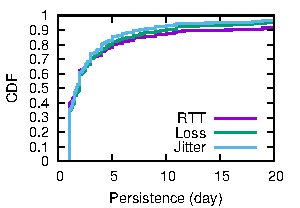
\includegraphics[width=0.45\textwidth]{figures/Via-Persistence-AsPair.pdf}
        \label{subfig:temporal-structure-persistence}
}
\subfloat[\small{Prevalence}]
{
        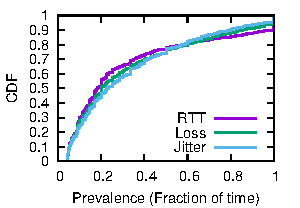
\includegraphics[width=0.45\textwidth]{figures/Via-Prevalence-AsPair.pdf}
        \label{subfig:temporal-structure-prevalence}
}
\caption{Temporal patterns of poor network performance. 
Figure~\ref{subfig:temporal-structure-persistence} and 
\ref{subfig:temporal-structure-prevalence} show the distribution of 
the persistence and prevalence of AS pairs having high PNR.}
\label{fig:temporal-structure}
\end{figure}





\subsection{Temporal Patterns}
\label{subsec:measurement:voip:temporal}

We now analyze temporal patterns of poor network 
performance. 
We perform this analysis by grouping the 
performance of AS pairs into $24$-hour time 
windows.\footnote{Different grouping granularities
yielded similar observations.}
We conservatively label an AS pair as having 
{\em high PNR} for a specific metric (on a given day) if 
its PNR on that day is at least $50\%$ higher than the 
overall PNR of all calls on that day. 

%Knowing what types of calls are more likely to have poor performance, however, does not mean they can be easily fixed. Next, we study the spatial and temporal patterns of bad network performance, and show that fixing a handful of AS pairs in specific time periods does not address most of them, which suggests the needs for a system that can adaptively alleviate bad network performance for users all over the world.

%\myparatight{Methodology} To understand the spatial and temporal patterns of bad network performance, we consider the performance distribution of each AS pair within different time windows of 24 hours. We first group the calls based on the pair of source and destination AS, and to ensure statisical significance, we consider each AS pair that have at least 20 calls in each day\footnote{We decide to group calls by source and destination AS pair on a daily base because it is the finest granularity that still have enough calls for most of the time. We used different grouping granularities and found qualitatively similar observations.}. 
%\ga{Let's see if we can argue for AS-level analysis as reasonable. Maybe present some /24 granularity data, show that the trends are similar when there is sufficient data, and say we will use AS-level data owing to the density? As we have all discussed before, it is not a natural granularity to pick unless we say why so.}

Figure~\ref{subfig:temporal-structure-persistence} and 
\ref{subfig:temporal-structure-prevalence} show the 
distribution of {\em persistence} and {\em prevalence} of 
high PNR AS-pairs. 
The {\em persistence} of an AS pair is the median 
number of consecutive days when it has high PNR. 
The {\em prevalence} of an AS pair is the fraction of 
time it has high PNR.
The figures show a highly skewed distribution with 
$10\%-20\%$ AS pairs always having high PNR, while 
$60\%-70\%$ AS pairs have poor performance for less 
than $30\%$ of time and lasting no longer than one 
day at a stretch. 
%These majority of AS pairs whose poor network performance is neither prevalent nor persistent should be improved in a dynamic manner.
%This means the poor performance of most AS pairs is neither prevalent nor persistent.
%This means that to fix the majority of AS pairs that are neither prevalent nor persistent that statically configuring a solution to improve only the (relatively few) most prevalent and persistent AS pairs is not sufficient; 
This observation suggests that instead of statically 
configuring the system to improve performance for 
only the (relatively few) most prevalent and persistent 
AS pairs, we need to dynamically decide if a call 
should use default Internet routing or be relayed. % sent through overlays.
%It reinforces the point 
%, in order to improve performance for the majority of AS pairs. 


\subsection{Cross-Metric Correlations}
\label{subsec:measurement:voip:correlation}

As there could be dependencies between network 
metrics, improving one metric may increase PNR of another 
metric. 
Figure~\ref{fig:perf-correlation} shows the three pair-wise 
correlations. 
While the plot is based on an aggregation of data across all 
calls and paths, the substantial spread suggests at least the 
possibility that improving one performance metric {\em could} 
lead to a worsening of the other metrics. 
Therefore, we also focus on reducing PNR of three metrics 
collectively, i.e., minimizing how often {\em at least one} of 
the metrics is poor.

\begin{figure}[t!]
\centering
\subfloat[\small{RTT vs. loss rate}]
{
        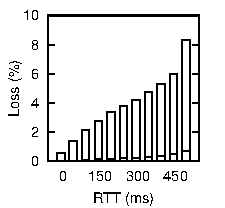
\includegraphics[width=0.3\textwidth]{figures/Via-Quality-Correlation-RTT-loss.pdf}
        \label{subfig:}
}
\subfloat[\small{RTT vs. jitter}]
{
        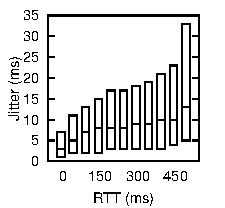
\includegraphics[width=0.3\textwidth]{figures/Via-Quality-Correlation-RTT-jitter.pdf}
        \label{subfig:}
}
\subfloat[\small{Jitter vs. loss rate}]
{
        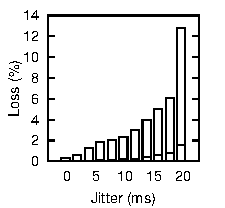
\includegraphics[width=0.3\textwidth]{figures/Via-Quality-Correlation-jitter-loss.pdf}
        \label{subfig:}
}
\caption{Pair-wise correlation between performance metrics. 
The Y-axis shows the distribution ($10^{\text{th}}$, $50^{\text{th}}$, 
$90^{\text{th}}$ percentiles) of one metric as a function the other 
metric over the same set of calls.}
%\ga{Only 25th, median, 90th? Also jitter vs. loss}
\label{fig:perf-correlation}
\end{figure}




%\subsection{Discussion}
%%\subsection{Key Observations}
%\label{subsec:measurement:voip:discuss}
%
%The key observations from this section are:
%\begin{enumerate}
%\item {\em Network performance matters.} User experience of 
%calls is impacted by even small changes in network metrics. 
%\item {\em Wide-area} communication, such as international 
%and inter-domain calls, are more prone to bad network performance, 
%and have a large room of improvement.
%\item Calls suffering from poor networks are spread {\em spatially} 
%(across ASes) and {\em temporally}. 
%%Most calls with poor network performance are not from a handful of source-destination AS pairs. And most source-destination pairs only experience high PNR for a relatively short period of time.
%\end{enumerate}

%These observations motivate the need for a network overlay (Observation 1) that provides better paths with a {\em global} footprint of overlay nodes (Observation 2), and the need to choose routes {\em selectively} and {\em dynamically} (Observation 3). 
